\section{Local orbital frame}
\label{sec:local}

\begin{itemize}
    \item[-] \textbf{Give the definition of a geocentric inertial reference frame}

    \textit{Geocentric} refers to the centre of the reference frame being the centre of the Earth. 
    Reference frames can typically be divided into \textit{inertial} and \textit{non-inertial} reference frames, where \textit{inertial} means that the frame is not accelerating (or rotating) and is fixed. 
    The orientation of the coordinate axes is fixed relative to distant stars, typically defined by the vernal equinox and the celestial equator.
    Such frames are more often used due to simplification of the calculation of motion laws.
    
    An example of an often-used geocentric inertial reference frame is the Earth-Centric Inertial (ECI).
    
    \item[-] \textbf{Give the definition of the local orbital frame $R_{LOF}$}
    
    A local orbit reference frame Z-, Y- and X-axis are defined as follows:
    \begin{itemize}
        \item $Z_{ol}$ or \textbf{R}: points directly from the centre of the central body (in this case Earth) towards the orbiting object (in this case the satellite), Zenith direction.
        
        \item $Y_{ol}$ or \textbf{W}: points in the direction of the normal positive to the orbital plane.
    
        \item $X_{ol}$ or \textbf{S}: completes the orthonormal trihedron and in this case points in the direction of the satellite's movement along its orbit.
    \end{itemize} 
    
    \begin{figure}[h]
        \centering
        \subfloat[From lecture slides, (R,S,W) vectors (1-2-3)]
        {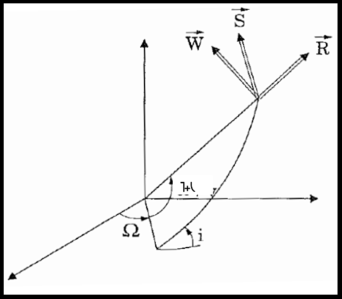
\includegraphics[width=0.4\textwidth]{Graphics/cloe_LOF.png}
        \label{fig:f2-1}}
        %\hfill
        \subfloat[qsw local orbital reference frame]
        {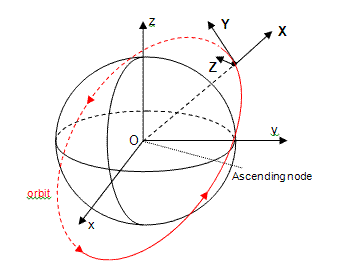
\includegraphics[width=0.45\textwidth]{Graphics/qsw_frame.png}
        \label{fig:f2-2}}
        \caption{The LOF axis can be defined in different ways, such as in (b), where it is the X-axis that follows the radial or zenith direction \cite{ISAE_frames}}
    \end{figure}
    
    
    \newpage
    \item[-] \textbf{Compute the Cubesat local orbital frame vector directions in your geocentric reference frame RE (theoretical computation)}
    
    To compute the LOF vector directions we first define the local orbital frame in Python according to the above-mentioned (R,W,S) definition.
    Then, we define a position vector, \textit{r}, and a velocity vector, \textit{v}, in the geocentric reference frame.
    The LOF unit vectors are defined mathematically according to the position and velocity vectors and their sizes (normalised):
    \begin{itemize}
        \item $\vec{R} = \frac{\vec{r}}{|r|}$ \qquad \qquad (radial component)
        \item $\vec{W} = \vec{R} \times \vec{V}$ \qquad (normal component)
        \item $\vec{S} = \frac{\vec{v}}{|v|}$ \qquad \qquad (tangential component)
    \end{itemize}

    An example of these vectors is generated in the Python code on lines 20-29 with the output:
    \begin{lstlisting}[frame=single, language=Python]
        Radial Direction (R_hat): [1. 0. 0.]
        Normal Direction (W_hat): [0. 0. 1.]
        Tangential Direction (S_hat): [0. 1. 0.]
    \end{lstlisting}

    
    
    \item[-] \textbf{Make a plot of the local orbital frame vector directions (as a function of time)}

    plot...

    refer to python code in appendix?

    

\end{itemize}